\subsection{Chaotic system under study}  \label{sec:chaos}

The  family of $2D$-quadratic maps studied here are modelled by a pair of coupled quadratic equations:

\begin{equation}\label{eq:mapaSprott}
 \left\{\begin{aligned}
        x_{n+1}&=a_1+a_2 x_n+a_3 x_n^2+a_4 x_n y_n+a_5 y_n+a_6 y_n^2\\
        y_{n+1}&=a_7+a_8 x_n+a_9 x_n^2+a_{10} x_n y_n+a_{11} y_n+a_{12} y_n^2
       \end{aligned}
 \right.
\end{equation}

where $\{x,y\}$ are the state variables and $\{a_i, i=1,\dots,12\}$
are the parameters. 
The main characteristic of this system is it presents multiple chaotic attractors depending on the selected
point in the parameter's space. The $12D$ parameters space generated by coefficients $A=\{a_1,...,a_{12}\}$  is very hard to be explored. \\
The reasons to study this particular system are two-fold: 

\begin{enumerate}
\item Using floating-point arithmetic Sprott saw
that by automatic swept of parameters $a_i$ a huge number of
points in the parameter's space (about $6  .  10^{16}$) having
a chaotic permanent regime may be detected. He also
found a correlation between the correlation dimension and the
Lyapunov exponents of these chaotic attractors, with their
\textsl{visual appeal}, an interesting issue for automatic
\textsl{art} generation.
\item It is possible to employ them in a wide variety of electronic applications, such as generate novel encryption systems either by replacing the S-box in AES \cite{Ahmad2013,Hussain2013}, or even by developing new encryption algorithms \cite{Machado2004,Smaoui2009}. 
\end{enumerate}

Three of these chaotic attractors are shown together in Fig. \ref{fig:atractores}. Their parameters sets $A_i$ are:
%
\begin{align*}
A_1&=\{-0.7,-0.4,0.5,-1.0,-0.9,-0.8,0.5,0.5,0.3,0.9,-0.1,-0.9\},\nonumber\\
A_2&=\{-0.6,-0.1,1.1,0.2,-0.8,0.6,-0.7,0.7,0.7,0.3,0.6,0.9\}, \nonumber\\
A_3&=\{ -0.1,0.8,-0.7,-1.1,1.1,-0.7,-0.4,0.6,-0.6,-0.3,1.2,0.6\}.\nonumber\\
\end{align*}
%
As it can be seen in the figure it is possible to get very different outputs just modifying the value of the parameters and maintaining the structure of the system. In an electronic implementation this would be equivalent to keeping the hardware structure and by modifying the parameters through, for example, an input it would be possible to vary the output.

Figures \ref{fig:atractores3592}.a to \ref{fig:atractores3592}.d show the same three attractors $A_1$ to $A_3$ of Fig. \ref{fig:atractores} and together with attractor $A_4=\{-1,0.9,0.4,-0.2,-0.6,-0.5,0.4,0.7,0.3,-0.5,0.7,-0.8\}$, superimposed with their basins of attraction (in grey).  The white areas of each figure correspond to those initial conditions generating divergent trajectories of the system (useless seeds regarding their use as PRNGs).

%%=========================ATRACTORES 3, 5 y 9 JUNTOS =======================================
\begin{figure}
    \centering
     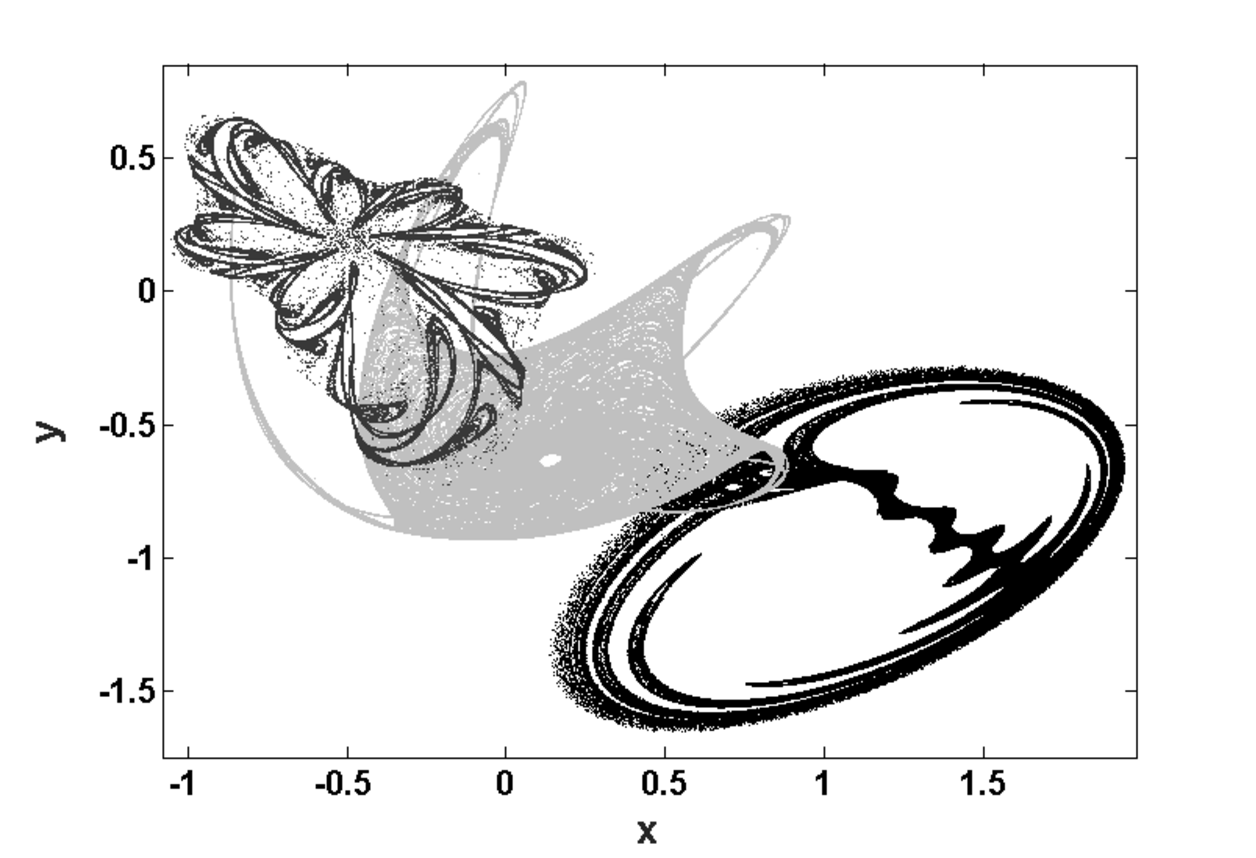
\includegraphics[width=1\columnwidth]{atractoreslindos}\\
    \caption{Three attractors for three different sets of  coefficients of $2D$-quadratic map.}\label{fig:atractores}
\end{figure}
%===========================================================================================

\begin{figure}
    \centering
    \begin{subfigure}[b]{0.49\textwidth}
        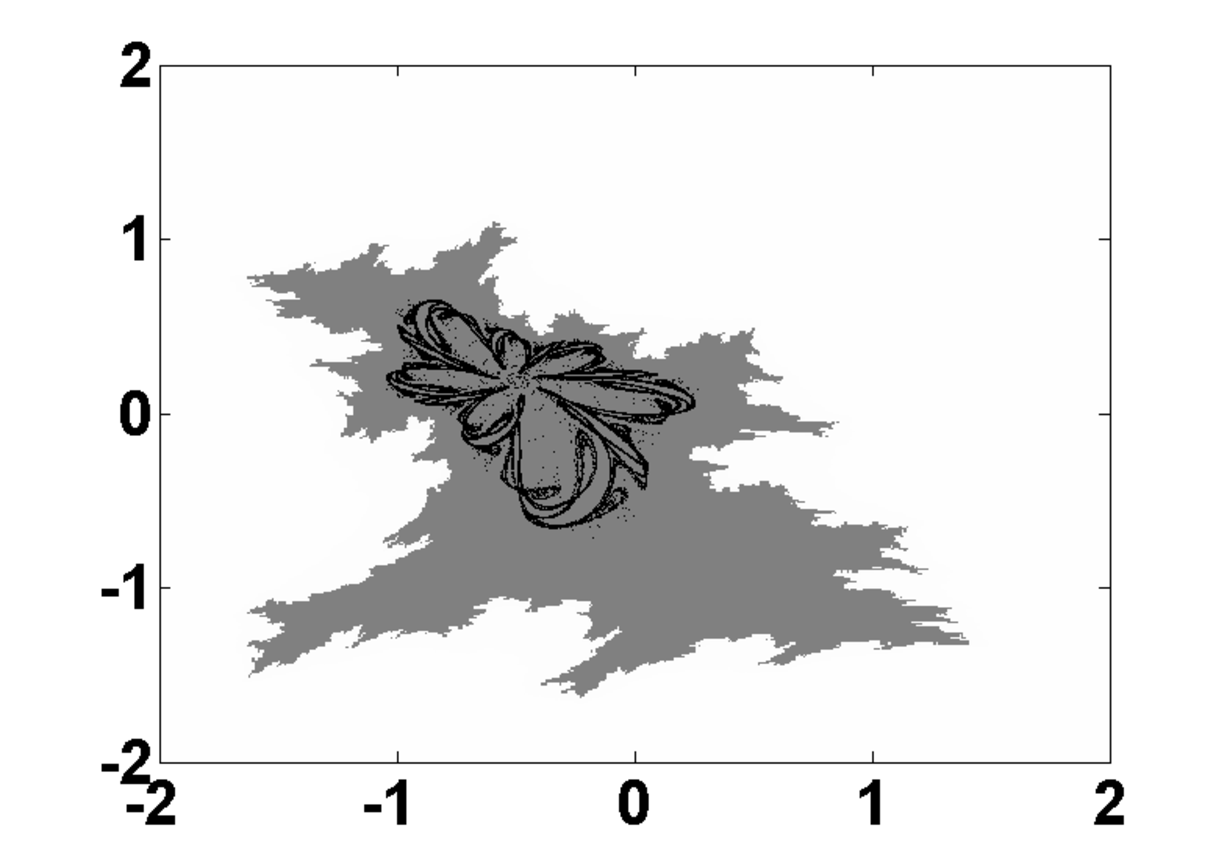
\includegraphics[width=\textwidth]{Atractor3_condominio}
        \caption{$\{a_i\}=A_1$.}
        \label{fig:gull}
    \end{subfigure}
    \hfill 
    \begin{subfigure}[b]{0.49\textwidth}
        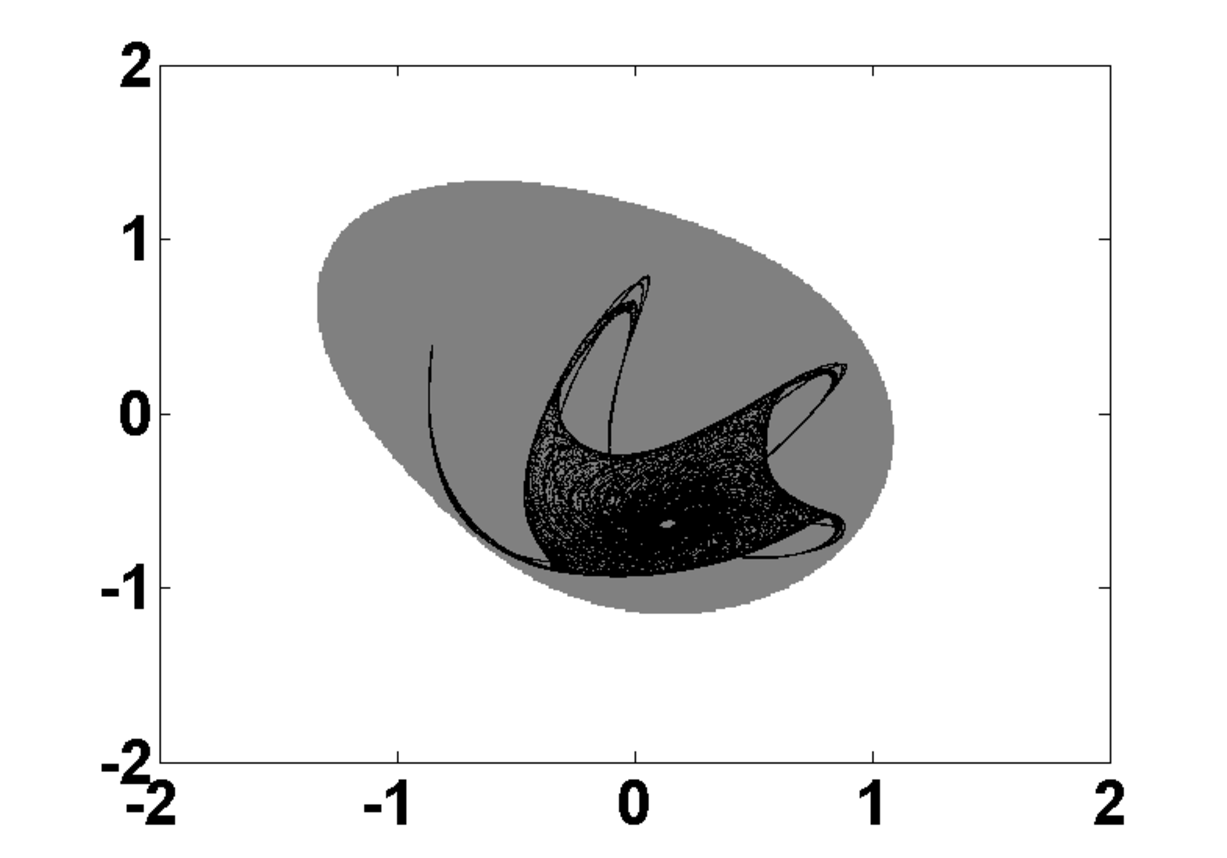
\includegraphics[width=\textwidth]{Atractor5_condminio}
        \caption{$\{a_i\}=A_2$.}
        \label{fig:tiger}
    \end{subfigure}
   \hfill 
    \begin{subfigure}[b]{0.49\textwidth}
        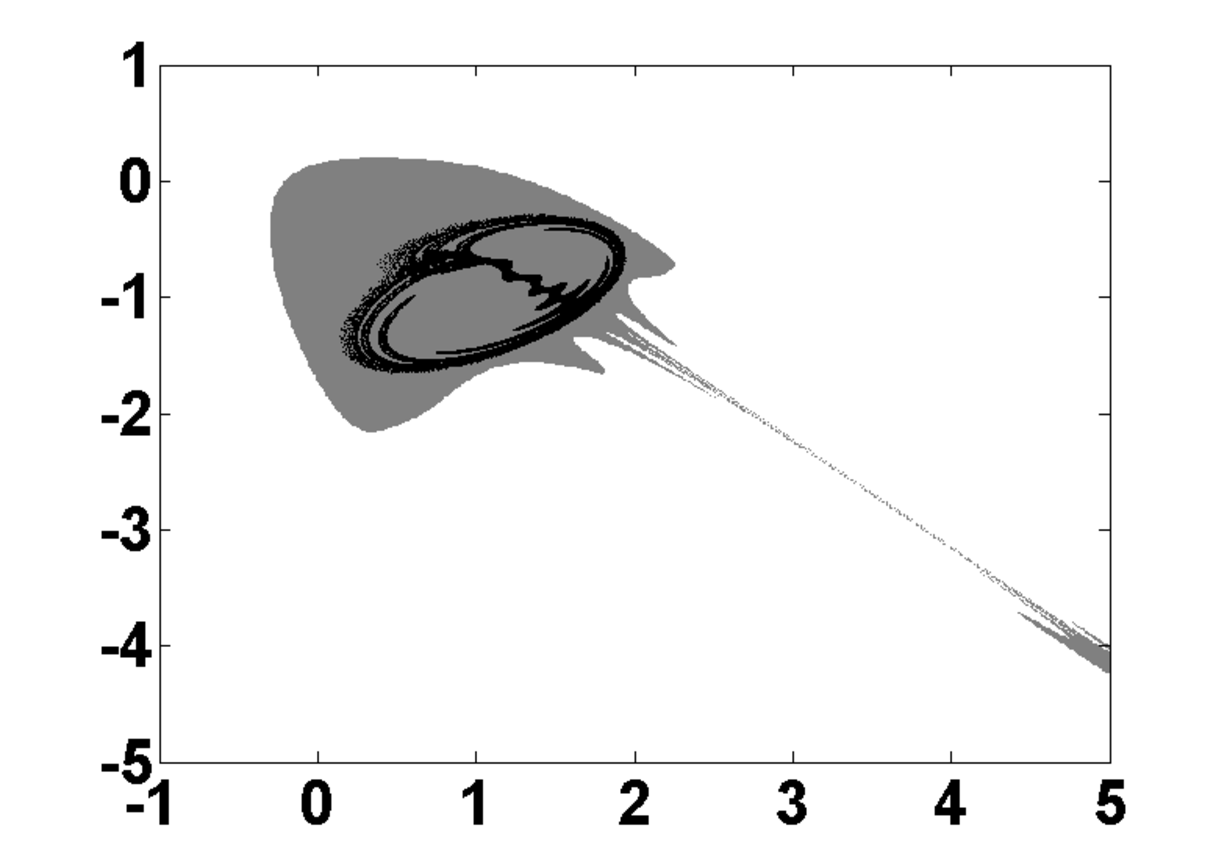
\includegraphics[width=\textwidth]{Atractor9_condominio}
        \caption{$\{a_i\}=A_3$.}
        \label{fig:mouse}
    \end{subfigure}
  \hfill  
    \begin{subfigure}[b]{0.49\textwidth}
        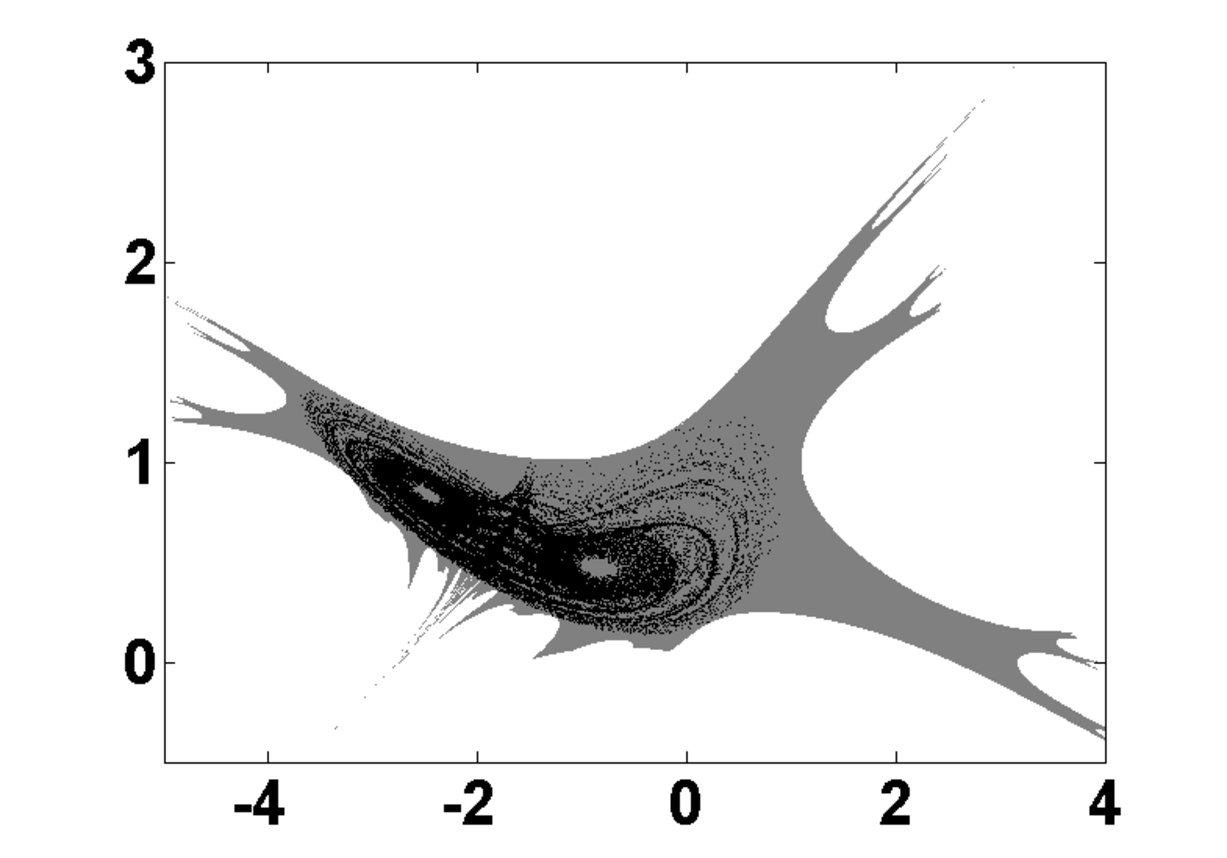
\includegraphics[width=\textwidth]{Atractor2_condominio}
        \caption{$\{a_i\}=A_4$.}
        \label{fig:mouse}
    \end{subfigure}
    \caption{Four chaotic attractors and their domains of attraction in floating-point arithmetics.}\label{fig:atractores3592}
\end{figure}